\documentclass[conference]{IEEEtran}
\usepackage{amsmath,amssymb}
\usepackage{graphicx}
\usepackage{booktabs}
\usepackage{tikz}
\usetikzlibrary{arrows.meta,positioning,fit}
\usepackage[hidelinks]{hyperref}
\usepackage{balance}

\newcommand{\sys}{FleetSentinel}

\begin{document}

\title{\sys{}: Population-Level Behavioral Monitoring for Detecting Rogue LLM Agents in Large-Scale Deployments}

\author{\IEEEauthorblockN{Dheeraj Arremsetty}
\IEEEauthorblockA{dheeraj.arremsetty@gmail.com}
\and
\IEEEauthorblockN{Co-Author Name~1}
\IEEEauthorblockA{affiliation\\email@example.com}
\and
\IEEEauthorblockN{Co-Author Name~2}
\IEEEauthorblockA{affiliation\\email@example.com}}

\maketitle

\begin{abstract}
Large language model (LLM) agents deployed at scale can be hijacked by indirect prompt injection and other attacks, causing them to execute actions their operators never intended. Existing runtime defenses monitor each agent in isolation, often with a second LLM in the loop, which is costly at fleet scale and, as we show, vulnerable to mimicry. We present \sys{}, a security layer that monitors a \emph{fleet} of LLM agents using two complementary, purely statistical signals: an \emph{individual} score comparing each episode's actions against a task-conditioned behavioral fingerprint over an argument-aware action alphabet, and a \emph{population} score measuring how unusual an episode is relative to the concurrent behavior of same-role peer agents. Per-agent evidence is aggregated sequentially across episodes with thresholds calibrated to an explicit fleet-level false-alarm budget. We evaluate \sys{} on 13{,}360 real execution traces (49{,}046 tool calls) produced by six LLMs on the AgentDojo benchmark, using episodes in which an injected task was actually executed as ground-truth rogue behavior. The combined score achieves ROC-AUC 0.76--0.82 per role (rising to 0.83 in the travel role once attacks with no observable action are excluded) and transfers to backbone models that contributed no profile data (mean 0.78 under leave-one-model-out), and in trace-grounded fleet simulations of 1{,}000--10{,}000 agents, \sys{} detects 96\% of persistent rogue agents within 20 episodes and 100\% within 50, at a $\approx$1\% agent-level false-alarm rate and $\sim$0.01\,ms of compute per episode. Against a mimicry attacker that constrains its episodes to evade individual fingerprinting, individual-evidence detection degrades from 0.60 to 0.40 while population-level evidence is essentially unaffected (0.92 vs.\ 0.90), supporting cross-agent baselining as a necessary complement to per-agent monitoring. We also delineate what action-level monitoring cannot see: injection goals achievable purely through the agent's text reply are statistically indistinguishable from benign episodes (ROC-AUC 0.56).
\end{abstract}

\begin{IEEEkeywords}
LLM agents, agent security, anomaly detection, prompt injection, behavioral fingerprinting, runtime monitoring
\end{IEEEkeywords}

\section{Introduction}
LLM-based agents that call tools---sending email, moving money, editing files---are moving from demonstrations to production fleets in which one operator runs hundreds or thousands of agent instances against shared infrastructure. This shift changes the security problem. A single agent that is hijacked by indirect prompt injection~\cite{greshake2023} or that misgeneralizes its instructions can take harmful, state-changing actions; benchmarks show that current models comply with injected tasks in a non-trivial fraction of episodes~\cite{debenedetti2024agentdojo,andriushchenko2025agentharm}. At fleet scale, the operator's question is no longer only ``was this output safe?'' but ``\emph{which of my ten thousand agents is no longer behaving like the others?}''

Existing runtime defenses largely monitor each agent in isolation. Guardrail systems such as LlamaFirewall~\cite{chennabasappa2025llamafirewall} and GuardAgent~\cite{xiang2024guardagent} interpose classifiers or a second LLM on each agent's inputs, reasoning, or tool calls; trace-analysis systems such as TraceAegis~\cite{traceaegis2025} and AgentArmor~\cite{agentarmor2025} check an agent's execution trace against rules or profiles derived from its own history. These designs share two costs. First, per-decision inference (often another LLM call) is expensive when multiplied across a fleet. Second, any detector calibrated only on an agent's \emph{own} normal behavior invites the classic mimicry strategy from intrusion detection~\cite{wagner2002mimicry}: an adversary who keeps each individual episode within the agent's normal envelope evades the monitor.

This paper argues that fleet-scale deployments make available a defense signal that single-agent monitors cannot use: \emph{the concurrent behavior of many agents operating in the same role}. If one banking agent among hundreds starts issuing transfers to a payee no peer has ever used, that deviation is visible in population statistics even when the episode looks unremarkable against the agent's own fingerprint. We design and evaluate \sys{}, a security layer built on this observation.

\subsection*{Contributions}
\begin{enumerate}
    \item \textbf{Design.} A monitoring architecture that combines (i) task-conditioned behavioral fingerprints over an \emph{argument-aware action alphabet}, scored with a bounded KL-divergence statistic, (ii) a population score computed by local-outlier-factor analysis over fleet snapshots, and (iii) sequential per-agent evidence aggregation with thresholds calibrated by bootstrap to an explicit fleet-level false-alarm budget. No LLM is invoked in the detection path.
    \item \textbf{Evaluation on real traces.} Using 13{,}360 published execution traces from six LLMs on AgentDojo~\cite{debenedetti2024agentdojo}, with episodes in which the injected task was actually executed as ground truth, the combined score reaches ROC-AUC 0.76--0.82 per role, outperforming allowlist rules, isolation forests, and one-class SVMs.
    \item \textbf{Fleet-scale and adversarial analysis.} In trace-grounded simulations of up to 10{,}000 agents, \sys{} detects 96\% of persistent rogue agents within 20 episodes (100\% within 50) at a $\approx$1\% agent-level false-alarm rate and $\sim$0.01\,ms per episode. A mimicry attacker that evades individual fingerprinting leaves population-level detection essentially unaffected; a low-and-slow attacker degrades detection in proportion to how much it throttles its own activity.
    \item \textbf{Scope delineation.} We show empirically that injection goals achievable purely through the agent's text reply (e.g., biased recommendations) are invisible to action-level monitoring (ROC-AUC 0.56), and we state this as a boundary of the approach rather than claiming coverage.
\end{enumerate}

\section{Related Work}
\textbf{Runtime guardrails for LLM agents.} LlamaFirewall~\cite{chennabasappa2025llamafirewall} combines prompt-injection classifiers with chain-of-thought auditing; GuardAgent~\cite{xiang2024guardagent} uses a second ``guard'' LLM that reasons over safety requests; AgentArmor~\cite{agentarmor2025} applies program analysis to runtime traces with a type system for data-flow policies. All operate per agent and most require model inference per decision. \sys{} differs in both unit of analysis (the fleet) and cost model (statistical scoring only); it is complementary to input-side defenses, which reduce the compromise rate that the sentinel then monitors.

\textbf{Anomaly detection on agent traces.} TraceAegis~\cite{traceaegis2025} abstracts stable execution units from an agent's history and validates traces against hierarchical and behavioral rules; SentinelAgent~\cite{sentinelagent2025} monitors multi-agent systems as dynamic execution graphs with an LLM-powered oversight agent. Both profile the monitored system's own behavior. \sys{} adds the cross-agent dimension---to our knowledge the first evaluation of population-level baselining for LLM agent fleets---and quantifies why it matters: it is the component that survives mimicry (Sec.~\ref{sec:exp3}).

\textbf{Benchmarks and attacks.} AgentDojo~\cite{debenedetti2024agentdojo} provides tool-using agent tasks with realistic prompt-injection attack cases and machine-checked outcomes; AgentHarm~\cite{andriushchenko2025agentharm} measures agent misuse; Greshake et al.~\cite{greshake2023} introduced indirect prompt injection; Wei et al.~\cite{wei2023jailbroken} analyze why safety training fails under jailbreaks. We use AgentDojo traces as evaluation data because its per-episode security labels indicate whether the injected task was \emph{actually executed}---exactly the ``rogue behavior'' event a runtime monitor must catch.

\textbf{Classical behavioral intrusion detection.} Our design consciously inherits from host-based anomaly detection: system-call profiling~\cite{forrest1996sense}, mimicry attacks~\cite{wagner2002mimicry}, and standard novelty detectors---LOF~\cite{breunig2000lof}, isolation forests~\cite{liu2008isolation}, one-class SVMs~\cite{scholkopf2001estimating}. The fleet setting revives an option that host-based IDS rarely had: a large population of peers executing the same role concurrently.

\section{Threat Model}\label{sec:threat}
\textbf{System.} An operator runs $N$ agent instances (potentially heterogeneous backbone models) partitioned into \emph{roles}: groups configured with the same tools and task distribution (e.g., ``banking assistant''). Agents interact with the environment exclusively through logged tool calls; the sentinel observes tool names and arguments but does not inspect model weights or (in this work) natural-language content.

\textbf{Adversary.} The adversary controls content the agent ingests (documents, emails, web pages, tool outputs) and seeks to make the agent execute attacker-chosen tasks: exfiltrating data via tool calls, moving money, modifying state, or derailing the agent. The adversary may adapt: it may throttle how often compromised episodes occur (low-and-slow) and may prefer injected tasks whose action footprint resembles normal behavior (mimicry). We assume the adversary does not control a majority of the fleet simultaneously (population statistics assume rogue behavior is rare at any instant), and cannot tamper with the sentinel or its logs.

\textbf{Out of scope.} (i) Attacks achieving their goal purely through the agent's \emph{text reply} with no unnecessary tool call---we show these are statistically invisible to action-level monitoring and require content-aware defenses; (ii) supply-chain compromise of the agent software itself; (iii) collusion of a large fraction of the fleet, which degrades the population baseline.

\section{Design}\label{sec:design}

\begin{figure}[t]
\centering
\resizebox{\linewidth}{!}{%
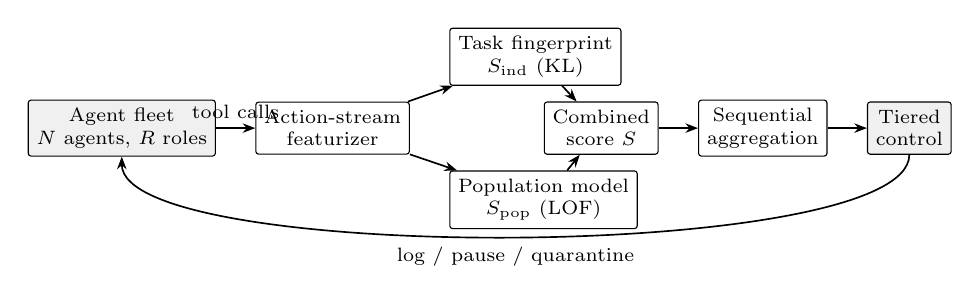
\begin{tikzpicture}[
    font=\scriptsize,
    box/.style={draw, rounded corners=1pt, align=center, inner sep=3pt, minimum height=5.5mm},
    arr/.style={-{Stealth[length=1.6mm]}, semithick},
    node distance=3.5mm and 5mm]
  \node[box, fill=gray!12, minimum width=17mm] (fleet) {Agent fleet\\$N$ agents, $R$ roles};
  \node[box, right=of fleet] (feat) {Action-stream\\featurizer};
  \node[box, above right=2mm and 5mm of feat] (ind) {Task fingerprint\\$S_{\mathrm{ind}}$ (KL)};
  \node[box, below right=2mm and 5mm of feat] (pop) {Population model\\$S_{\mathrm{pop}}$ (LOF)};
  \node[box, right=17mm of feat] (comb) {Combined\\score $S$};
  \node[box, right=of comb] (seq) {Sequential\\aggregation};
  \node[box, right=of seq, fill=gray!12] (ctl) {Tiered\\control};
  \draw[arr] (fleet) -- node[above]{tool calls} (feat);
  \draw[arr] (feat) -- (ind);
  \draw[arr] (feat) -- (pop);
  \draw[arr] (ind) -- (comb);
  \draw[arr] (pop) -- (comb);
  \draw[arr] (comb) -- (seq);
  \draw[arr] (seq) -- (ctl);
  \draw[arr] (ctl.south) to[out=-90, in=-90, looseness=0.35] node[below]{log / pause / quarantine} (fleet.south);
\end{tikzpicture}}
\caption{\sys{} architecture. Each episode's tool-call stream is scored against a task-conditioned fingerprint (individual evidence) and against the concurrent behavior of same-role peers (population evidence); per-agent evidence accumulates across episodes and drives tiered control.}
\label{fig:arch}
\end{figure}

\subsection{Setting and notation}
An \emph{episode} is one assigned task executed by one agent: a sequence of tool calls $a_1,\dots,a_n$, each with a tool name and arguments. Episodes from agents in the same role are assumed exchangeable when benign. For each role, the operator retains a small set of \emph{profile runs}: logged benign episodes per assigned task (in deployment, from a staging period or early supervised operation).

\subsection{Task-conditioned fingerprints over an argument-aware alphabet}\label{sec:fingerprint}
A naive fingerprint---the role's marginal distribution over tool names---fails in practice: a hijacked agent usually still performs most of its assigned task, so tool \emph{frequencies} barely move (Sec.~\ref{sec:exp1} measures this directly). The signal lies in \emph{which arguments} calls carry and in what the \emph{assigned task} makes necessary. \sys{} therefore conditions on the assigned task and extends the action alphabet with argument novelty.

From the profile runs we identify \emph{identifier-like} argument fields: (tool, key) pairs whose values recur across benign runs with low diversity (payees, account numbers, cities, file IDs), as opposed to free-text fields (subjects, message bodies) whose values are model-generated and vary run to run. Field $(f,k)$ is identifier-like if it occurs $\ge 3$ times in profile runs with (distinct values)/(occurrences) $\le 0.5$. Each call then maps to a symbol:
\[
\sigma(a) =
\begin{cases}
f\#\mathrm{novel} & \parbox[t]{0.6\linewidth}{if tool $f$ is absent from the task profile, or any identifier-like argument value was never observed in profile runs of this task or role,}\\[1ex]
f & \text{otherwise.}
\end{cases}
\]
The fingerprint $P_{r,t}$ is the smoothed (Laplace, $\alpha{=}0.5$) distribution of symbols in profile runs of task $t$ in role $r$; symbols of the form $f\#\mathrm{novel}$ never occur in profile runs and receive only smoothing mass. For an episode with empirical symbol distribution $Q$, the individual score is the bounded statistic
\begin{equation}
S_{\mathrm{ind}} \;=\; 1 - \exp\!\big(-D_{\mathrm{KL}}(Q \,\|\, P_{r,t})\big) \;\in\; [0,1),
\label{eq:sind}
\end{equation}
which specifies the normalization left open in score-fusion designs: injected calls surface as near-zero-probability symbols and drive $D_{\mathrm{KL}}$~\cite{kullback1951} up sharply, while smoothing keeps it finite. Tasks without profile runs fall back to the role-level fingerprint.

\subsection{Population score over fleet snapshots}\label{sec:population}
Each episode is embedded as a feature vector: its symbol distribution; log counts of calls, distinct tools, out-of-vocabulary tools, and tool errors; and its novel-action rate. Given a \emph{fleet snapshot}---the recent episodes of all agents in a role---\sys{} standardizes features within the snapshot and computes each episode's local outlier factor~\cite{breunig2000lof} ($k{=}35$ neighbors), mapped to
\begin{equation}
S_{\mathrm{pop}} = 1 - \exp\!\big(-\max(\mathrm{LOF}-1,\,0)\big) \in [0,1).
\label{eq:spop}
\end{equation}
This is deliberately \emph{unsupervised over the current population}: it requires no labels and no per-agent history, and it is the component an individual-mimicry adversary cannot influence without also changing what the rest of the fleet is doing. (An earlier design sketch used DBSCAN distance-to-centroid; DBSCAN yields no centroids, and density-based LOF is the appropriate formalization.)

\subsection{Combined score and sequential evidence}\label{sec:sequential}
The episode score is $S = w\,S_{\mathrm{ind}} + (1-w)\,S_{\mathrm{pop}}$, with $w$ a tuned hyperparameter; we sweep it rather than fixing it a priori and find $w^\ast \in [0.1, 0.5]$ across roles (Sec.~\ref{sec:exp1}), i.e., population evidence carries the majority of the weight everywhere.

Single episodes rarely justify intervention at fleet-acceptable false-alarm rates. \sys{} therefore maintains per-agent evidence: after an agent's $k$-th episode, its running mean $\bar S_k$ is compared against a threshold $\tau_k$ obtained by bootstrap over benign profile scores such that a benign agent's probability of ever being flagged over the monitoring horizon stays within the operator's budget $\beta$ (we use $\beta{=}1\%$). Control is tiered on the accumulated evidence: episodes with high $S$ are logged for audit; an agent whose $\bar S_k$ crosses $\tau_k$ is paused pending human review; confirmation quarantines the agent and rolls back its recent side effects where the tool layer supports it. Fingerprints are \emph{anchored to the profile runs} and are not updated from live traffic, so a patient adversary cannot drift them.

\subsection{Scalability}
Detection involves only counting, a KL sum over a small alphabet, and a $k$-NN density query in a $\sim$30-dimensional space---no model inference. Roles shard naturally across sentinel nodes; population snapshots are per-role and bounded. We measure $\sim$0.01\,ms of single-core compute per episode at snapshot sizes up to $10^4$ (Sec.~\ref{sec:exp2}), so a commodity core sustains $\sim$$10^5$ episodes/s---monitoring is a negligible fraction of the cost of running the agents themselves.

\section{Evaluation}\label{sec:eval}

\subsection{Dataset and ground truth}\label{sec:dataset}
We use the published execution traces of the AgentDojo benchmark~\cite{debenedetti2024agentdojo}: 13{,}360 episodes (49{,}046 tool calls) produced by six LLMs (three Claude, two GPT-4o, one Gemini, one Llama variant) across four suites, which we treat as roles: banking, Slack, travel, and workspace. Each attacked episode carries a machine-checked label indicating whether the injected task was \emph{actually executed}. This yields three classes: \textbf{benign} episodes with no injection present (582); \textbf{resisted} episodes where an attack was present but the agent stayed on task (10{,}116)---used as \emph{hard negatives}, since the malicious content appears in the agent's observations but not its behavior; and \textbf{compromised} episodes where the agent executed the injected task (2{,}662), spanning 15 attack styles. Reading each injected goal, we further classify compromised episodes as \emph{overt} (the goal requires at least one observable tool call: transfers, emails, deletions, posts) or \emph{covert} (achievable purely in the text reply); only travel's ``recommend this hotel'' goal is covert (67 episodes).

Per role, benign episodes are split 50/50 (stratified by model) into profile runs and test data; the test set is the held-out benign plus all resisted and compromised episodes. Population scores are computed over snapshots consisting of all test negatives plus compromised episodes subsampled to 2\% contamination, averaged over 30 draws.

\subsection{Experiment 1: detecting compromised episodes}\label{sec:exp1}

\begin{table}[t]
\caption{Episode-level detection (ROC-AUC) per role. PR-AUC in parentheses. Positives = compromised episodes; negatives = held-out benign + resisted.}
\label{tab:exp1}
\centering
\scriptsize
\setlength{\tabcolsep}{3.5pt}
\begin{tabular}{lcccc}
\toprule
Method & Banking & Slack & Travel & Workspace \\
\midrule
Role-level KL (naive) & .34 (.24) & .50 (.48) & .60 (.17) & .39 (.08) \\
Task-cond.\ KL ($S_{\mathrm{ind}}$) & .77 (.51) & .75 (.68) & .65 (.14) & .66 (.14) \\
Allowlist rule & .50 (.31) & .62 (.62) & .58 (.16) & .50 (.11) \\
Isolation forest & .70 (.45) & .58 (.53) & .54 (.11) & .58 (.12) \\
One-class SVM & .77 (.51) & .80 (.82) & .60 (.18) & .56 (.15) \\
Population LOF ($S_{\mathrm{pop}}$) & .68 (.48) & .78 (.49) & .76 (.21) & .70 (.25) \\
\textbf{Combined $S$} & \textbf{.82} (.51) & \textbf{.81} (.61) & \textbf{.76} (.20) & \textbf{.76} (.25) \\
\midrule
Combined, overt only & .82 & .81 & \textbf{.83} & .76 \\
Combined, covert only & --- & --- & \textbf{.56} & --- \\
\bottomrule
\end{tabular}
\end{table}

\begin{figure}[t]
\centering
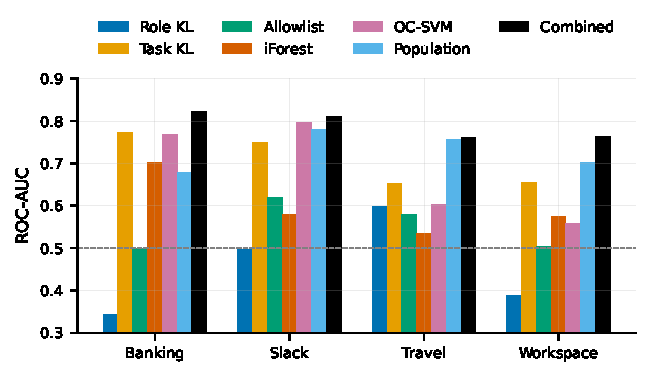
\includegraphics[width=\linewidth]{figures/auc_by_method.pdf}
\caption{Episode-level ROC-AUC by method and role.}
\label{fig:auc}
\end{figure}

Table~\ref{tab:exp1} and Fig.~\ref{fig:auc} summarize episode-level results. Three findings matter for design. \textbf{(1) Naive frequency fingerprints fail.} The role-level KL score is at or below chance in three roles: a hijacked agent still performs most of its assigned task, so marginal tool frequencies barely move---and benign episodes of \emph{unusual} tasks look more anomalous than compromised episodes of common ones. Task conditioning plus the argument-aware alphabet lifts the same statistic by up to 0.43 AUC (banking .34$\to$.77). \textbf{(2) Population evidence is the strongest single signal} in the two roles with the most diverse benign behavior (travel .76, workspace .70) and is competitive elsewhere; the combined score is best or tied-best in all four roles (.76--.82). \textbf{(3) Coverage is bounded by observability.} Restricted to overt attacks, combined AUC is .76--.83 (travel, the only role with covert attacks, improves from .76 to .83); on the covert ``just say it'' goal it is .56, i.e., indistinguishable from noise---the empirical basis for the scope boundary in Sec.~\ref{sec:threat}. Attacks that derail the agent into inaction (DoS-style) also produce weak action-level signatures at strict operating points; utility monitoring, not anomaly detection, is the natural countermeasure there.

Single-episode operating points are modest: at 5\% episode-level FPR, the combined score catches 13--22\% of compromised episodes. This motivates the sequential design---the sentinel's unit of decision is the \emph{agent}, not the episode.

\textbf{Generalization to unseen backbone models.} A fleet operator will deploy agents on models that contributed no profile data. We therefore repeat detection in a leave-one-model-out protocol: for each of the six backbones, fingerprints and the population fleet context are built exclusively from the other five, and detection is evaluated on the held-out model's episodes. Mean combined-score ROC-AUC over the 19 model-role cells with $\ge$5 positives is \textbf{0.78}, on par with the in-fleet 0.76--0.82; on the held-out model with the most compromised episodes (GPT-4o; 139--703 positives per role) per-role AUC is 0.76--0.90. Behavioral baselines thus transfer across backbones: what the sentinel profiles is the \emph{role}, not the model.

\begin{figure}[t]
\centering
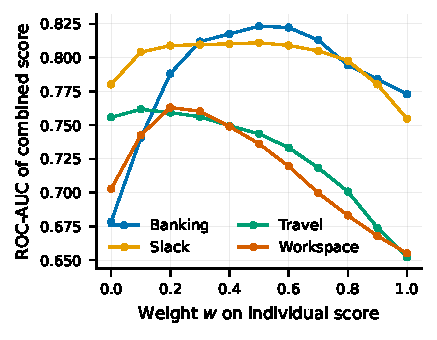
\includegraphics[width=0.78\linewidth]{figures/weight_sweep.pdf}
\caption{Combined-score AUC vs.\ weight $w$ on $S_{\mathrm{ind}}$. Optima lie at $w \le 0.5$ in all roles: population evidence carries the majority of the weight.}
\label{fig:sweep}
\end{figure}

\subsection{Experiment 2: fleet-scale sequential detection}\label{sec:exp2}
We simulate fleets of 1{,}000--10{,}000 agents (roles balanced, 1\% rogue) over a 100-episode horizon, drawing each benign agent's episode scores from the empirical negative-score distribution of its role and each rogue agent's from the empirical compromised (overt) distribution---i.e., the simulation's primitive quantities are real measured scores, not parametric assumptions. Thresholds $\tau_k$ are bootstrap-calibrated per role to a 1\% agent-level false-alarm budget.

\begin{figure}[t]
\centering
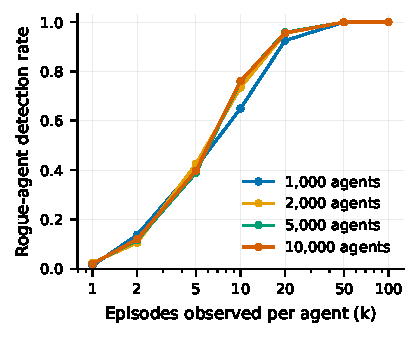
\includegraphics[width=0.8\linewidth]{figures/fleet_detection.pdf}
\caption{Fleet simulation: fraction of persistent rogue agents flagged vs.\ episodes observed, at a calibrated $\approx$1\% agent-level false-alarm rate. Curves are stable from 1k to 10k agents.}
\label{fig:fleet}
\end{figure}

Fig.~\ref{fig:fleet} shows the result: 76\% of persistent rogue agents are flagged within 10 episodes, 96\% within 20, and 100\% within 50, with realized agent-level false-alarm rates of 0.8--1.2\%; median detection latency is 10 episodes. Detection curves are essentially invariant from 1k to 10k agents. Measured population-scoring cost is 0.005--0.03\,ms per episode across snapshot sizes (near-linear scaling; Fig.~\ref{fig:thru}), and individual scoring adds $\sim$0.02\,ms.

\begin{figure}[t]
\centering
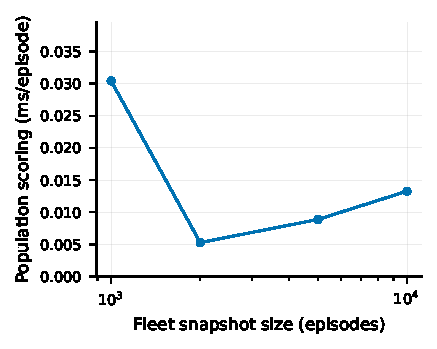
\includegraphics[width=0.75\linewidth]{figures/throughput.pdf}
\caption{Measured population-scoring cost per episode vs.\ snapshot size (single core).}
\label{fig:thru}
\end{figure}

\subsection{Experiment 3: adaptive adversaries}\label{sec:exp3}

\textbf{Low-and-slow.} A rogue agent that is compromised only in a fraction $p$ of its episodes dilutes the evidence stream. Fig.~\ref{fig:lowslow} quantifies the trade-off: at $p{=}0.5$, 98\% of rogue agents are still caught within 100 episodes; at $p{=}0.2$, 44\%; at $p \le 0.1$, most evade the horizon. The defense implication is honest but useful: throttling to evade \sys{} costs the adversary a 5--20$\times$ reduction in malicious activity, and longer horizons continue to accumulate evidence.

\begin{figure}[t]
\centering
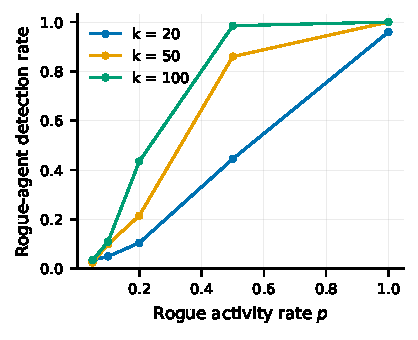
\includegraphics[width=0.75\linewidth]{figures/low_and_slow.pdf}
\caption{Low-and-slow adversary: detection vs.\ rogue activity rate $p$ after $k$ episodes.}
\label{fig:lowslow}
\end{figure}

\textbf{Mimicry.} We model an adversary that restricts compromised episodes to those whose \emph{individual} score already evades the per-episode individual threshold (95th percentile of benign)---a strong assumption in the attacker's favor, and easy to satisfy: 88--97\% of real compromised episodes qualify. Fig.~\ref{fig:mimicry} shows agent-level detection at $k{=}20$ under three evidence types. Individual-only detection degrades from 0.60 to 0.40; population-only detection is essentially unchanged (0.92 $\to$ 0.90); the combined detector remains at 0.96--0.97. The population signal survives because these episodes, while within the agent's own normal envelope, still involve argument values and action patterns that are \emph{rare across the fleet}---the property the attacker cannot control without controlling the fleet.

\begin{figure}[t]
\centering
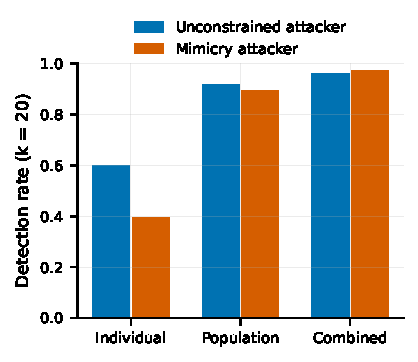
\includegraphics[width=0.75\linewidth]{figures/mimicry.pdf}
\caption{Mimicry adversary constrained to evade individual fingerprinting: population-level evidence is essentially unaffected.}
\label{fig:mimicry}
\end{figure}

\section{Discussion and Limitations}\label{sec:limits}
\textbf{What the sentinel cannot see.} Action-level monitoring has a principled blind spot: attacks achieving their goal entirely in the text channel (covert AUC .56). Content-aware signals---output classifiers, taint tracking from untrusted inputs to replies---are the complementary defense; \sys{} reduces, but does not eliminate, reliance on them. DoS-style derailment similarly manifests as \emph{absence} of action, better caught by utility monitoring.

\textbf{Adversarial residual.} A sufficiently patient adversary ($p \le 0.1$) can stay under the sequential test within our 100-episode horizon, and a fleet-wide compromise (e.g., a poisoned shared tool) would shift the population baseline itself, blinding $S_{\mathrm{pop}}$; anchored fingerprints and cross-role consistency checks mitigate but do not remove this.

\textbf{External validity.} AgentDojo's four suites are realistic but narrow, its episodes are short ($\sim$3.7 calls on average), and our fleet simulation assumes episodes are drawn i.i.d.\ from per-role score distributions---real fleets exhibit workload drift and task-mix shifts that would require periodic re-profiling and threshold re-calibration. Profile runs must themselves be clean; poisoned profiles are an open supply-chain risk. Finally, our per-role episode populations (hundreds to thousands) are far smaller than production fleets; larger populations should \emph{improve} LOF density estimates, but this remains to be demonstrated.

\section{Conclusion}
\sys{} reframes rogue-agent detection as a fleet problem. Two inexpensive statistical signals---task-conditioned fingerprints over an argument-aware action alphabet, and population-level outlier analysis across same-role peers---suffice to flag 96\% of persistently compromised agents within 20 episodes at a 1\% false-alarm budget and microsecond-scale per-episode cost, on real traces from six models. The population signal, unavailable to single-agent monitors, is precisely the component that survives mimicry. We make our pipeline available for reproduction and see two natural next steps: integrating content-aware signals to close the covert-channel gap, and a live pilot in a production agent platform.

\section*{Acknowledgments and Declarations}
\textit{Author contributions:} D.A.\ conceived the framework, performed the experiments, and wrote the manuscript. [Co-author contributions to be added.] \textit{Funding:} none. \textit{Data:} all traces are from the publicly released AgentDojo runs~\cite{debenedetti2024agentdojo}; experiment code is available from the author on request.

\balance
\begin{thebibliography}{20}

\bibitem{greshake2023}
K.~Greshake, S.~Abdelnabi, S.~Mishra, C.~Endres, T.~Holz, and M.~Fritz,
``Not what you've signed up for: Compromising real-world LLM-integrated
applications with indirect prompt injection,'' in \emph{Proc.\ 16th ACM
Workshop on Artificial Intelligence and Security (AISec)}, 2023.

\bibitem{debenedetti2024agentdojo}
E.~Debenedetti, J.~Zhang, M.~Balunovi\'c, L.~Beurer-Kellner, M.~Fischer, and
F.~Tram\`er, ``AgentDojo: A dynamic environment to evaluate prompt injection
attacks and defenses for LLM agents,'' in \emph{Advances in Neural Information
Processing Systems 37 (NeurIPS), Datasets and Benchmarks Track}, 2024.

\bibitem{andriushchenko2025agentharm}
M.~Andriushchenko \emph{et~al.}, ``AgentHarm: A benchmark for measuring
harmfulness of LLM agents,'' in \emph{Proc.\ Int.\ Conf.\ on Learning
Representations (ICLR)}, 2025.

\bibitem{chennabasappa2025llamafirewall}
S.~Chennabasappa \emph{et~al.}, ``LlamaFirewall: An open source guardrail
system for building secure AI agents,'' \emph{arXiv:2505.03574}, 2025.

\bibitem{xiang2024guardagent}
Z.~Xiang \emph{et~al.}, ``GuardAgent: Safeguard LLM agents by a guard agent
via knowledge-enabled reasoning,'' \emph{arXiv:2406.09187}, 2024.

\bibitem{traceaegis2025}
B.~Ruan \emph{et~al.}, ``TraceAegis: Securing LLM-based agents via
hierarchical and behavioral anomaly detection,'' \emph{arXiv:2510.11203},
2025.

\bibitem{sentinelagent2025}
X.~He \emph{et~al.}, ``SentinelAgent: Graph-based anomaly detection in
multi-agent systems,'' \emph{arXiv:2505.24201}, 2025.

\bibitem{agentarmor2025}
P.~Wang \emph{et~al.}, ``AgentArmor: Enforcing program analysis on agent
runtime trace to defend against prompt injection,'' \emph{arXiv:2508.01249},
2025.

\bibitem{wei2023jailbroken}
A.~Wei, N.~Haghtalab, and J.~Steinhardt, ``Jailbroken: How does LLM safety
training fail?'' in \emph{Advances in Neural Information Processing Systems 36
(NeurIPS)}, 2023.

\bibitem{wagner2002mimicry}
D.~Wagner and P.~Soto, ``Mimicry attacks on host-based intrusion detection
systems,'' in \emph{Proc.\ 9th ACM Conf.\ on Computer and Communications
Security (CCS)}, 2002.

\bibitem{forrest1996sense}
S.~Forrest, S.~A. Hofmeyr, A.~Somayaji, and T.~A. Longstaff, ``A sense of self
for Unix processes,'' in \emph{Proc.\ IEEE Symp.\ on Security and Privacy},
1996.

\bibitem{breunig2000lof}
M.~M. Breunig, H.-P. Kriegel, R.~T. Ng, and J.~Sander, ``LOF: Identifying
density-based local outliers,'' in \emph{Proc.\ ACM SIGMOD Int.\ Conf.\ on
Management of Data}, 2000.

\bibitem{liu2008isolation}
F.~T. Liu, K.~M. Ting, and Z.-H. Zhou, ``Isolation forest,'' in \emph{Proc.\
8th IEEE Int.\ Conf.\ on Data Mining (ICDM)}, 2008.

\bibitem{scholkopf2001estimating}
B.~Sch\"olkopf, J.~C. Platt, J.~Shawe-Taylor, A.~J. Smola, and R.~C.
Williamson, ``Estimating the support of a high-dimensional distribution,''
\emph{Neural Computation}, vol.~13, no.~7, pp. 1443--1471, 2001.

\bibitem{kullback1951}
S.~Kullback and R.~A. Leibler, ``On information and sufficiency,''
\emph{Annals of Mathematical Statistics}, vol.~22, no.~1, pp. 79--86, 1951.

\end{thebibliography}

\end{document}
